% \documentclass[12pt,english,ignorenonframetext,aspectratio=169,]{beamer}
\documentclass[11pt,english,ignorenonframetext,]{beamer}

%%%%%%%%%%%%%%%
%% Beamer theme
% choose one from http://deic.uab.es/~iblanes/beamer_gallery/
% or http://www.hartwork.org/beamer-theme-matrix/
% \usetheme{Warsaw}
\usetheme{CambridgeUS}

%%%%%%%%%%%%%%%%%%%%%%
%% Beamer color theme
%% default albatross beaver beetle crane dolphin dove fly lily
%% orchid rose seagull seahorse whale wolverine

%\usecolortheme{seahorse}  %% very lighty
\usecolortheme{dolphin}    %% nice blue
\usecolortheme{orchid}     %% dark red ?
\usecolortheme{whale}      %% black and blue as Warsaw

%%%%%%%%%%%%%%%%%%%%%%%%%%%%%%%%%%%%%%%%%%%%%%%%%%%%%%%%%%%%%%%%%%%%%%%%%%%%%%%%
%% Change the theme
%\setbeamercolor{alerted text}{fg=orange}
%\setbeamercolor{background canvas}{bg=white}
%\setbeamercolor{block body alerted}{bg=normal text.bg!90!black}
%\setbeamercolor{block body}{bg=normal text.bg!90!black}
%\setbeamercolor{block body example}{bg=normal text.bg!90!black}
%\setbeamercolor{block title alerted}{use={normal text,alerted text},fg=alerted text.fg!75!normal text.fg,bg=normal text.bg!75!black}
%\setbeamercolor{block title}{bg=blue}
%\setbeamercolor{block title example}{use={normal text,example text},fg=example text.fg!75!normal text.fg,bg=normal text.bg!75!black}
%\setbeamercolor{fine separation line}{}
\setbeamercolor{frametitle}{fg=black}
%\setbeamercolor{item projected}{fg=black}
%\setbeamercolor{normal text}{bg=black,fg=yellow}
%\setbeamercolor{palette sidebar primary}{use=normal text,fg=normal text.fg}
%\setbeamercolor{palette sidebar quaternary}{use=structure,fg=structure.fg}
%\setbeamercolor{palette sidebar secondary}{use=structure,fg=structure.fg}
%\setbeamercolor{palette sidebar tertiary}{use=normal text,fg=normal text.fg}
%\setbeamercolor{section in sidebar}{fg=brown}
%\setbeamercolor{section in sidebar shaded}{fg= grey}
\setbeamercolor{separation line}{}
%\setbeamercolor{sidebar}{bg=red}
%\setbeamercolor{sidebar}{parent=palette primary}
%\setbeamercolor{structure}{bg=black, fg=green}
%\setbeamercolor{subsection in sidebar}{fg=brown}
%\setbeamercolor{subsection in sidebar shaded}{fg= grey}
%\setbeamercolor{title}{fg=blackblue}
%\setbeamercolor{titlelike}{fg=blackblue}


%%%%%%%%%%%%%%%%%%%%%%%
%% Other beamer options
% \setbeamercovered{transparent}
\setbeamercovered{invisible}
% Permet de laisser en gris le texte qui n'est pas encore apparu (lorsqu'on utilise les commandes avec des <1,2> ou <4-9>.

%\setbeamercolor{normal text}{fg=black,bg=white}

%%%%%%%%%%%%%%%%%%%%%%%
%% Change Beamer fonts
% \usefonttheme{default}
% \usefonttheme[onlymath]{serif}
\usefonttheme{serif}

\setbeamerfont{title}{family=\rm}
\setbeamerfont{titlelike}{family=\rm}
\setbeamerfont{frametitle}{family=\rm}

%%%%%%%%%%%%%%%%%%%%%%%%%%%%%%%%%%%%%%%%%%%%%%%%%%%%%%%%%%%%%%%%%%%%%%%%%%%%%%%%
%% innertheme
%% rectangles circles inmargin rounded
% \useinnertheme{rounded}  % XXX My preference
\useinnertheme{circles}    % XXX

%%%%%%%%%%%%%%%%%%%%%%%%%%%%%%%%%%%%%%%%%%%%%%%%%%%%%%%%%%%%%%%%%%%%%%%%%%%%%%%%
%% outertheme
%% infolines miniframes shadow sidebar smoothbars smoothtree split tree
%\useoutertheme{infolines}

%% No navigation symbol.
\setbeamertemplate{navigation symbols}{}
\beamertemplatenavigationsymbolsempty

% XXX Add a background image to the slides
% \usepackage{tikz}
% \setbeamertemplate{background}{
\includegraphics[width=\paperwidth,height=\paperheight,keepaspectratio]{IETR.jpg}}
% \setbeamertemplate{background}{{\centering\begin{tikzpicture}\node[opacity=0.15]{
\includegraphics[width=0.98\paperwidth]{IETR_et_partenaires_IETR.png}};\end{tikzpicture}}}

% Other options
%\setbeamertemplate{footline}[page number]

\beamertemplateballitem
\setbeamertemplate{itemize item}[square]


\setbeamertemplate{caption}[numbered]
\setbeamertemplate{caption label separator}{: }
\setbeamercolor{caption name}{fg=normal text.fg}
\beamertemplatenavigationsymbolsempty
\usepackage{lmodern}
\usepackage{color}
  \newcommand{\urlb}[1]{\textcolor{blue}{\url{#1}}}
%% Color definition
\usepackage{xcolor}
%% WARNING attention when changing the colors, change both the {RGB}{r,g,b} and % rgb(r,g,b)
\definecolor{blackblue}{RGB}{19,19,59}  % rgb(48,48,150)
\definecolor{bleu}{RGB}{0,0,204}           % rgb(0,0,204)
\definecolor{deeppurple}{RGB}{102,0,204}   % rgb(102,0,204)
\definecolor{darkgreen}{RGB}{0,100,0}      % rgb(0,100,0)
\definecolor{yellowgreen}{RGB}{200,215,0}  % rgb(200,215,0)
\definecolor{bluegreen}{RGB}{0,185,140}    % rgb(0,185,140)
\definecolor{gold}{RGB}{255,180,0}         % rgb(255,180,0)
\definecolor{meca}{RGB}{255,110,0}         % rgb(255,110,0)
\definecolor{strongred}{RGB}{255,0,0}      % rgb(255,0,0)
\definecolor{normalred}{RGB}{204,0,0}      % rgb(204,0,0)
\definecolor{darkred}{RGB}{174,0,0}        % rgb(174,0,0)
\definecolor{info}{RGB}{174,0,0}        % rgb(174,0,0)
\definecolor{darkblue}{RGB}{0,0,174}        % rgb(0,0,174)
\definecolor{maths}{RGB}{0,0,174}        % rgb(0,0,174)
\definecolor{darkpurple}{RGB}{114,0,114}   % rgb(114,0,114)
\definecolor{ml}{RGB}{114,0,114}   % rgb(114,0,114)

\usepackage{amssymb,amsmath}
\usepackage{bbm,bm}  % bold maths symbols
\usepackage{ifxetex,ifluatex}
\usepackage{fixltx2e} % provides \textsubscript

% % FIXME remove as soon as possible, it slows down compilation to import TikZ
% %% TikZ
% \usepackage{tikz}
% \usetikzlibrary{snakes,arrows,shapes}
% % https://tex.stackexchange.com/a/226974/
% \tikzset{
%   font={\fontsize{10pt}{10}\selectfont}
% }
\usepackage{tikzsymbols}  % https://tex.stackexchange.com/a/227226/97964

\IfFileExists{macrosText.sty}{\usepackage{macrosText}}{}

\usepackage[linesnumbered,commentsnumbered,inoutnumbered,slide]{algorithm2e}


\ifnum 0\ifxetex 1\fi\ifluatex 1\fi=0 % if pdftex
  \usepackage[T1]{fontenc}
  \usepackage[utf8]{inputenc}
\else % if luatex or xelatex
  \ifxetex
    \usepackage{mathspec}
  \else
    \usepackage{fontspec}
  \fi
  \defaultfontfeatures{Ligatures=TeX,Scale=MatchLowercase}
\fi
% use upquote if available, for straight quotes in verbatim environments
\IfFileExists{upquote.sty}{\usepackage{upquote}}{}
% use microtype if available
\IfFileExists{microtype.sty}{%
\usepackage{microtype}
\UseMicrotypeSet[protrusion]{basicmath} % disable protrusion for tt fonts
}{}
\newif\ifbibliography
\hypersetup{
            pdfborder={0 0 0},
            breaklinks=true}
% \urlstyle{same}  % don't use monospace font for urls
% Code embedding.
\usepackage{palatino}              % Use the Palatino font % XXX remove if it is ugly ?
\usepackage{graphicx,grffile}
\makeatletter
\def\maxwidth{\ifdim\Gin@nat@width>\linewidth\linewidth\else\Gin@nat@width\fi}
\def\maxheight{\ifdim\Gin@nat@height>\textheight0.8\textheight\else\Gin@nat@height\fi}
\makeatother
% Scale images if necessary, so that they will not overflow the page
% margins by default, and it is still possible to overwrite the defaults
% using explicit options in \includegraphics[width, height, ...]{}
\setkeys{Gin}{width=\maxwidth,height=\maxheight,keepaspectratio}

\ifxetex
\usepackage{fontspec}
\setmainfont[Ligatures=Historic]{TeX Gyre Pagella}
\newfontfamily\FiraCode{Fira Code}
\setmonofont[Contextuals={Alternate}]{Fira Code}
\newfontfamily\Fontify[Path = ../common/]{Fontify-Regular}
\else
\newcommand{\Fontify}{}
\fi

% Prevent slide breaks in the middle of a paragraph:
\widowpenalties 1 10000
\raggedbottom

% \AtBeginPart{
%   \let\insertpartnumber\relax
%   \let\partname\relax
%   \frame{\partpage}
% }
% \AtBeginSection{
%   \ifbibliography
%   \else
%     \let\insertsectionnumber\relax
%     \let\sectionname\relax
%     \frame{\sectionpage}
%   \fi
% }
% % Si on veut faire apparaître le sommaire courant à chaque nouvelle section.
% \AtBeginSection{
%   \begin{frame}<beamer>%[t]
%   %\frametitle{Local outline}  % Translate the name of the slide
%   \frametitle{\hspace{0pt}}  % Translate the name of the slide
%     \begin{LARGE}  % XXX LARGE font for this slide?
%     \tableofcontents[currentsection, sectionstyle=show/hide, subsectionstyle=hide/hide]
%     \end{LARGE}  % XXX LARGE font for this slide?
%   \end{frame}
% }
% \AtBeginSubsection{
%   \let\insertsubsectionnumber\relax
%   \let\subsectionname\relax
%   \frame{\subsectionpage}
% }

\setlength{\parindent}{0pt}
\setlength{\parskip}{6pt plus 2pt minus 1pt}
\setlength{\emergencystretch}{3em}  % prevent overfull lines
\providecommand{\tightlist}{%
  \setlength{\itemsep}{0pt}\setlength{\parskip}{0pt}}
\setcounter{secnumdepth}{5}

% https://tex.stackexchange.com/a/70495/
\usepackage{appendixnumberbeamer}


% For \justifying command, see https://tex.stackexchange.com/a/148696/
\usepackage{ragged2e}
\addtobeamertemplate{frame begin}{}{\justifying}
\addtobeamertemplate{block begin}{}{\justifying}
\addtobeamertemplate{block alerted begin}{}{\justifying}
\addtobeamertemplate{block example begin}{}{\justifying}
\addtobeamertemplate{itemize body begin}{}{\justifying}
\addtobeamertemplate{itemize item}{}{\justifying}
\addtobeamertemplate{itemize subitem}{}{\justifying}
\addtobeamertemplate{itemize subsubitem}{}{\justifying}
\addtobeamertemplate{enumerate body begin}{}{\justifying}
\addtobeamertemplate{enumerate item}{}{\justifying}
\addtobeamertemplate{enumerate subitem}{}{\justifying}
\addtobeamertemplate{enumerate subsubitem}{}{\justifying}
\addtobeamertemplate{description body begin}{}{\justifying}
\addtobeamertemplate{description item}{}{\justifying}


\title[B-GLR test and Non-Stationary MAB]{The Bernoulli Generalized Likelihood Ratio test (B-GLR) for Non-Stationary Multi-Armed Bandits}
\subtitle{Research Seminar at PANAMA, IRISA lab, Rennes}

\author[Lilian Besson]{\Large \textbf{Lilian Besson}}

\institute[]{{\large
  PhD Student}{\newline
  % \normalsize
  \newline SCEE team, IETR laboratory, CentraleSupélec in Rennes
  \newline \& SequeL team, CRIStAL laboratory, Inria in Lille}}

\date{Thursday $6^{\text{th}}$ of June, $2019$}

\begin{document}
\justifying

\begin{frame}[plain]
  \titlepage

  % XXX manual inclusion of logos
  \begin{center}
    
\includegraphics[height=0.18\textheight]{../common/LogoIETR.png}
    
\includegraphics[height=0.21\textheight]{../common/LogoCS.png}
    
\includegraphics[height=0.18\textheight]{../common/LogoInria.jpg}
  \end{center}

\end{frame}


\begin{frame}{Publications associated with this talk}

  \begin{itemize}
    \item
      \href{https://hal.inria.fr/hal-02006471/document}{``Analyse non asymptotique d'un test séquentiel de détection de ruptures et application aux bandits non stationnaires''}\\
      by \textbf{L. Besson} \&
      \href{http://chercheurs.lille.inria.fr/ekaufman/research.html}{E.
      Kaufmann}

      $\hookrightarrow$ presented at the
      \textbf{GRETSI} conference, in Lille (France), next August 2019

    \vspace*{30pt}

    \item
      \href{https://hal.inria.fr/hal-02006471/document}{``The Generalized Likelihood Ratio Test meets klUCB: an Improved Algorithm for Piece-Wise Non-Stationary Bandits''}\\
      by \textbf{L. Besson} \&
      \href{http://chercheurs.lille.inria.fr/ekaufman/research.html}{E.
      Kaufmann}\\
      February 2019,
      pre-print on
      \href{https://hal.inria.fr/hal-02006471}{\textcolor{blue}{HAL-02006471}}
      and
      \href{https://arxiv.org/abs/1902.01575}{\textcolor{blue}{arXiv:1902.01575}}

  \end{itemize}

\end{frame}


\section{\hfill{}Outline of the talk\hfill{}}

\begin{frame}{Outline of the talk}

  \begin{enumerate}
    \item
      (Stationary) Multi-armed bandits problems
    \vspace*{15pt}

    \item
      Piece-wise stationary multi-armed bandits problems
    \vspace*{15pt}

    \item
      The B-GLR test and its finite time properties
    \vspace*{15pt}

    \item
      The BGLRT-klUCB algorithm
    \vspace*{15pt}

    \item
      Regret analysis
    \vspace*{15pt}

    \item
      Numerical simulations
  \end{enumerate}

\end{frame}


\section{\hfill{}1. (Stationary) Multi-armed bandits problems\hfill{}}

\begin{frame}{1. (Stationary) Multi-armed bandits problems}

  \begin{enumerate}
    \item
    \alert{\textbf{%
      (Stationary) Multi-armed bandits problems
    }}
    \vspace*{15pt}

    \item
    \textcolor{gray}{
      Piece-wise stationary multi-armed bandits problems
    }
    \vspace*{15pt}

    \item
    \textcolor{gray}{
      The B-GLR test and its finite time properties
    }
    \vspace*{15pt}

    \item
    \textcolor{gray}{
      The BGLRT-klUCB algorithm
    }
    \vspace*{15pt}

    \item
    \textcolor{gray}{
      Regret analysis
    }
    \vspace*{15pt}

    \item
    \textcolor{gray}{
      Numerical simulations
    }
  \end{enumerate}

\end{frame}

\subsection{\hfill{}What is a bandit problem?\hfill{}}

\begin{frame}{Multi-armed bandits}

  $=$ Sequential decision making problems in uncertain environments :

  \centering
  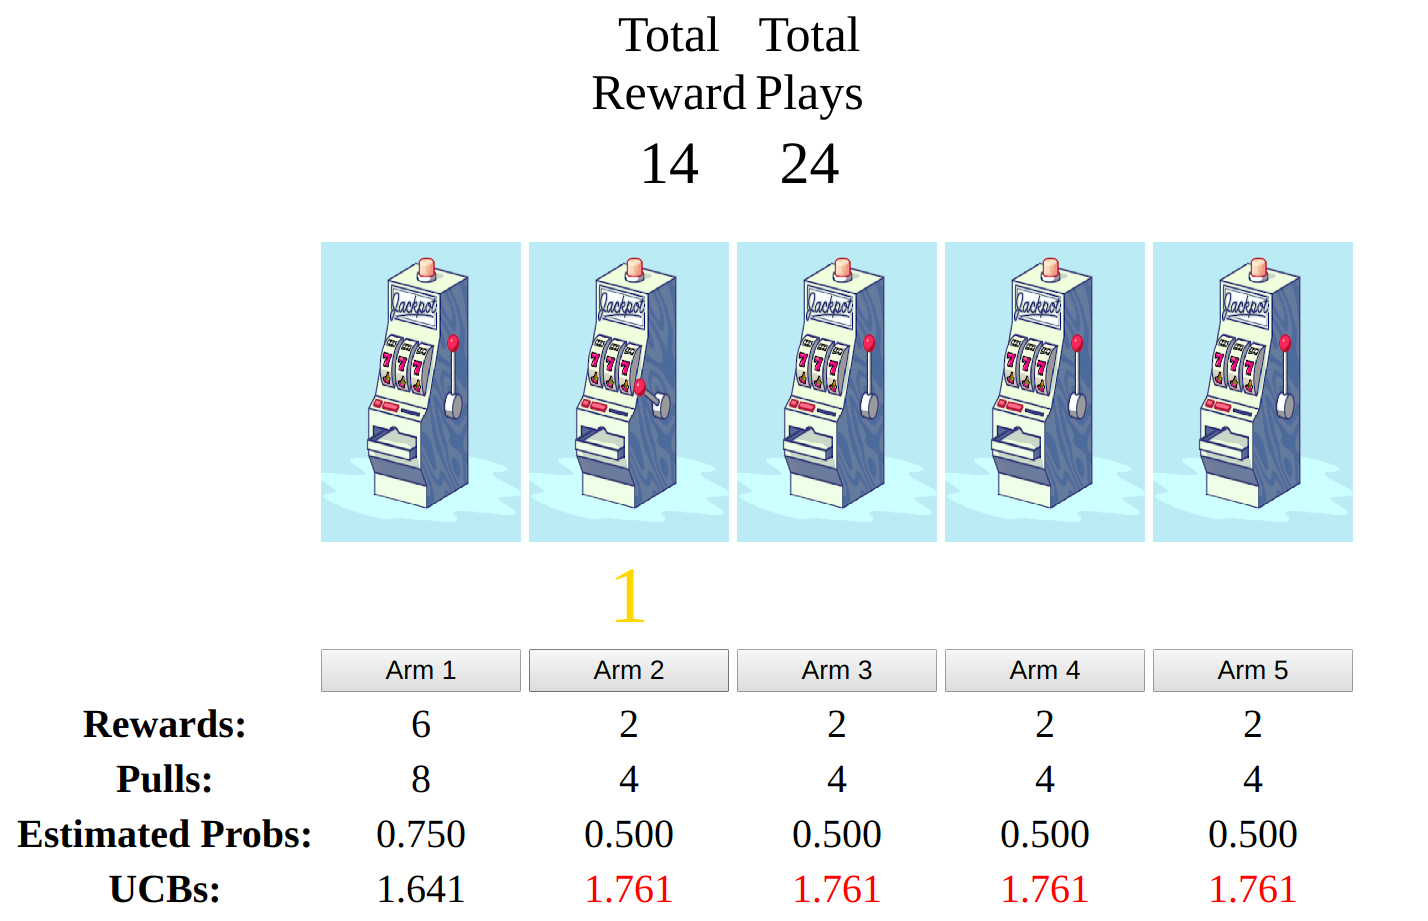
\includegraphics[height=0.65\textheight]{figures/example_of_a_5_arm_bandit_problem.png}

  {\tiny
  $\hookrightarrow$ Interactive demo
    \href{https://perso.crans.org/besson/phd/MAB_interactive_demo/}{\textcolor{blue}{\texttt{perso.crans.org/besson/phd/MAB\_interactive\_demo/}}}
  }

\end{frame}


\subsection{\hfill{}Mathematical model\hfill{}}

\begin{frame}{Mathematical model}

\begin{itemize}
  \item
  Discrete time steps $t = 1, \dots, T$\\
  The \emph{horizon} $T$ is fixed and usually unknown

  \item
  At time $t$, an \emph{agent plays the arm} $A(t)\in\{1,\dots,K\}$,\\
  then she observes the \emph{iid random reward} $r(t) \sim \nu_k$, $r(t)\in\mathbb{R}$

  \pause
  \item
  Usually, we focus on Bernoulli arms $\nu_k = \mathrm{Bernoulli}(\mu_k)$, of mean $\mu_k\in[0,1]$,
  giving binary rewards $r(t) \in\{0,1\}$.

  \pause
  \item
  \textbf{Goal} : maximize the sum of rewards $\sum\limits_{t=1}^T r(t)$

  \item
  or \alert{maximize the sum of expected rewards $\mathbb{E}\left[ \sum\limits_{t=1}^T r(t) \right]$}

  \pause
  \item
  Any efficient policy must balance \alert{between exploration and exploitation}:
  it must explore all arms to discover the best one,
  while exploiting the arms known to be good so far.
\end{itemize}

\end{frame}


\subsection{\hfill{}Naive solutions\hfill{}}

\begin{frame}{Two examples of bad solutions}

  \begin{exampleblock}{$i)$ Pure exploration}
    \begin{itemize}
      \item
      Play arm $A(t) \sim \mathcal{U}(\{1,\dots,K\})$ uniformly at random
      \item
      $\implies$ Mean expected rewards
      $ \frac{1}{T} \mathbb{E}\left[ \sum\limits_{t=1}^T r(t) \right] = \frac{1}{K} \sum\limits_{k=1}^K \mu_k \ll \mu^*$
    \end{itemize}
  \end{exampleblock}

  \pause

  \begin{exampleblock}{$ii)$ Pure exploration}
    \begin{itemize}
      \item
        Count the number of samples and the sum of rewards of each arm $N_k(t) = \sum\limits_{s < t} \bold{1}(A(s)=k)$ and $X_k(t) = \sum\limits_{s < t} r(s) \bold{1}(A(s)=k)$
      \item
        Estimate the \alert{unknown} mean $\mu_k$ with $\widehat{\mu_k}(t) = X_k(t) / N_k(t)$
      \item
        Play the arm of maximum empirical mean : $A(t) = \arg\max_k \widehat{\mu_k}(t)$
      \item
        Performance depends on the first draws, and can be very poor!
    \end{itemize}
  \end{exampleblock}

  {\tiny
    Interactive demo
    $\hookrightarrow$ \href{https://perso.crans.org/besson/phd/MAB_interactive_demo/}{\textcolor{blue}{\texttt{perso.crans.org/besson/phd/MAB\_interactive\_demo/}}}
  }

\end{frame}


\subsection{\hfill{}The \emph{``Upper Confidence Bound''} algorithm\hfill{}}

\begin{frame}{A first solution : the \emph{``Upper Confidence Bound''} algorithm}

  \begin{itemize}
    \item
      Compute $\mathrm{UCB}_k(t) = X_k(t) / N_k(t) + \sqrt{\alpha \log(t) / N_k(t)}$ \\
      $=$ an \alert{upper confidence bound} on the \alert{unknown} mean $\mu_k$
    \item
      Play the arm of maximal UCB : $A(t) = \arg\max_k \mathrm{UCB}_k(t)$
      \\
      $\hookrightarrow$ Principle of ``optimism under uncertainty''
    \item
      $\alpha$ balances between \emph{exploitation} ($\alpha\to0$) and \emph{exploration}  ($\alpha\to\infty$)

    \pause

    \item
      \alert{UCB is efficient}:
      the best arm is identified correctly (with high probability) if there are enough samples (for $T$ large enough)
    \item
      $\implies$
      Expected rewards attains the maximum
      ($\forall \alpha>1/2$)
      \[ \text{For~} T\to\infty, \;\;\; \frac{1}{T} \mathbb{E}\left[ \sum\limits_{t=1}^T r(t) \right] \to \max_k \mu_k \]
  \end{itemize}
\end{frame}

\begin{frame}{Elements of the proof for UCB algorithm}

  \begin{block}{Elements of proof of convergence (for $K$ Bernoulli arms)}
    \begin{itemize}[<+->]
      \item
        Suppose the first arm is the best:
        $\mu^* = \mu_1 > \mu_2 \geq \ldots \mu_K$
      \item
        $\mathrm{UCB}_k(t) = X_k(t) / N_k(t) + \sqrt{\alpha \log(t) / N_k(t)}$
      \item
        Hoeffding's inequality gives
        $\mathbb{P}(\mathrm{UCB}_k(t) < \mu_k(t)) \propto \frac{1}{t^{2 \alpha}}$\\
        $\implies$ the different $\mathrm{UCB}_k(t)$ are true ``Upper Confidence Bounds'' on the (unknown) $\mu_k$ (most of the times)
      \item
        And if a suboptimal arm $k>1$ is sampled, it implies
        $\mathrm{UCB}_k(t) > \mathrm{UCB}_1(t)$, but $\mu_k < \mu_1$:
        Hoeffding's inequality also proves that ``wrong ordering'' of the $\mathrm{UCB}_k(t)$ are unlikely
      \item
        We can prove that suboptimal arms $k$ are sampled about $o(T)$ times\\
        $\implies \mathbb{E}\left[ \sum\limits_{t=1}^T r(t) \right] \underset{T\to\infty}{\to} \mu^* \times \mathcal{O}(T) + \sum\limits_{k: \Delta_k>0} \mu_k \times o(T)$

        \alert{At which speed do we have this convergence?}
    \end{itemize}
  \end{block}

\end{frame}


\subsection{\hfill{}Regret of a bandit algorithm\hfill{}}

\begin{frame}{Measure the performance of an algorithm $\mathcal{A}$ with its mean regret $R_{\mathcal{A}}(T)$}

\begin{itemize}
  \item
  Difference in the accumulated rewards between an ``oracle'' and $\mathcal{A}$

  \item
  The ``oracle'' algorithm always plays the (unknown) best arm $k^* = \arg\max \mu_k$ (we note the best mean $\mu_{k^*} = \mu^*$)

  \item
  Maximize the sum of expected rewards
  $\Longleftrightarrow$ \alert{minimize the regret}
  %
  \[ \alert{ R_{\mathcal{A}}(T) } = \mathbb{E}\left[ \sum\limits_{t=1}^T r_{k^*}(t) \right] - \sum\limits_{t=1}^T \mathbb{E}\left[ r(t) \right] = T \mu^* - \sum\limits_{t=1}^T \mathbb{E}\left[ r(t) \right]. \]

\end{itemize}

\pause
\vspace*{10pt}

\begin{exampleblock}{Typical regime for stationary bandits (lower \& upper bounds)}
  \begin{itemize}
  \item
  No algorithm $\mathcal{A}$ can obtain a regret better than
  \hfill{}
  $R_{\mathcal{A}}(T) \geq \Omega(\log(T))$

  \item
  And an efficient algorithm $\mathcal{A}$ obtains
  \hfill{}
  $R_{\mathcal{A}}(T) \leq \mathcal{O}(\log(T))$
  \end{itemize}
\end{exampleblock}

\end{frame}


\begin{frame}{Regret of the UCB algorithm and another algorithm}

  For any problem with $K$ arms following Bernoulli distributions, of means $\mu_1,\dots,\mu_K \in[0,1]$, and optimal arm $k^*$, then

  \begin{exampleblock}{For the UCB algorithm}
    \begin{small}
      \[ R_T^{\mathrm{UCB}} \leq ( \sum_{\substack{k=1,\dots,K \\ \mu_k < \mu_{k^*}}} \frac{8}{(\mu_k - \mu_{k^*})} ) \log(T) + o(\log(T)) = \mathcal{O}\left( \alert{C(\mu_1,\dots,\mu_K)} \log(T) \right). \]
    \end{small}%
  \end{exampleblock}

  \begin{exampleblock}<2->{For the kl-UCB algorithm: a small regret upper-bound}
    \begin{small}
      \[ R_T^{\mathrm{kl}\text{-}\mathrm{UCB}} \leq ( \sum_{\substack{k=1,\dots,K \\ \mu_k < \mu_{k^*}}} \frac{(\mu_k - \mu_{k^*})}{\mathrm{kl}(\mu_k, \mu_{k^*})} ) \log(T) + o(\log(T)). \]
      If $\mathrm{kl}(x, y) = x \log(x/y) + (1-x) \log((1-x)/(1-y))$ is the binary relative entropy (Kullback-Leibler divergence of two Bernoulli of means $x$ and $y$)
    \end{small}%
  \end{exampleblock}

\end{frame}

% FIXME !

\begin{frame}{Main contributions of my PhD thesis}

  For different extensions of the classical model of stationary bandits\ldots{}

  \begin{itemize}
    \item
      A clean mathematical model
    \item
      We propose new algorithms\ldots{}
      \newline
      with a new theoretical analysis, we obtain new regret bounds\ldots{}
      \newline
      that can verified on numerical simulations\ldots{}
    \item
      $\implies$ We improve the state-of-the-art on the two aspects of theoretical and empirical performances!
  \end{itemize}

\end{frame}


\begin{frame}{Deux contributions principales de ma thèse}

\begin{exampleblock}{Bandits stationnaires (classiques) avec $K$ bras et $T$ étapes}
  \[ R_{\mathcal{A}}(T) = \mathcal{O}\left( K \log(T) \right). \]
\end{exampleblock}

\begin{block}<2->{1) Bandits \textbf{multi-joueurs décentralisé} \hspace*{40pt} \href{https://arxiv.org/abs/1711.02317}{[Besson et al, ALT, 2018]}}
  Si \alert{$M \leq K$ joueurs} jouent face au même problème de bandit, \alert{avec collisions} mais sans communication entre eux ni sans contrôle centralisé :
  %
  $R_{\mathrm{MCTopM}}(T) = \mathcal{O}\left( K \alert{M^3} \log(T) \right)$.
\end{block}

\begin{block}<3->{2) Bandits stationnaires \textbf{par morceaux} \hspace*{25pt} \href{https://arxiv.org/abs/1902.01575}{[Besson et al, GRETSI, 2019]}}
  Si le problème est \alert{stationnaire par morceaux, sur $\Upsilon = o(\sqrt{T})$ intervalles ``assez grands''} :
  %
  $R_{\mathrm{B}\text{-}\mathrm{GLR}}(T) = \mathcal{O}\left( K \sqrt{\alert{\Upsilon} T \log(T)} \right)$.
\end{block}

\end{frame}


\section{\hfill{}2. Piece-wise stationary multi-armed bandits problems\hfill{}}

\begin{frame}{2. Piece-wise stationary multi-armed bandits problems}

  \begin{enumerate}
    \item
    \textcolor{gray}{
      (Stationary) Multi-armed bandits problems
    }
    \vspace*{15pt}

    \item
    \alert{\textbf{%
      Piece-wise stationary multi-armed bandits problems
    }}
    \vspace*{15pt}

    \item
    \textcolor{gray}{
      The B-GLR test and its finite time properties
    }
    \vspace*{15pt}

    \item
    \textcolor{gray}{
      The BGLRT-klUCB algorithm
    }
    \vspace*{15pt}

    \item
    \textcolor{gray}{
      Regret analysis
    }
    \vspace*{15pt}

    \item
    \textcolor{gray}{
      Numerical simulations
    }
  \end{enumerate}

\end{frame}


\section{\hfill{}3. The B-GLR test and its finite time properties\hfill{}}

\begin{frame}{3. The B-GLR test and its finite time properties}

  \begin{enumerate}
    \item
    \textcolor{gray}{
      (Stationary) Multi-armed bandits problems
    }
    \vspace*{15pt}

    \item
    \textcolor{gray}{
      Piece-wise stationary multi-armed bandits problems
    }
    \vspace*{15pt}

    \item
    \alert{\textbf{%
      The B-GLR test and its finite time properties
    }}
    \vspace*{15pt}

    \item
    \textcolor{gray}{
      The BGLRT-klUCB algorithm
    }
    \vspace*{15pt}

    \item
    \textcolor{gray}{
      Regret analysis
    }
    \vspace*{15pt}

    \item
    \textcolor{gray}{
      Numerical simulations
    }
  \end{enumerate}

\end{frame}


\section{\hfill{}4. The BGLRT-klUCB algorithm\hfill{}}

\begin{frame}{4. The BGLRT-klUCB algorithm}

  \begin{enumerate}
    \item
    \textcolor{gray}{
      (Stationary) Multi-armed bandits problems
    }
    \vspace*{15pt}

    \item
    \textcolor{gray}{
      Piece-wise stationary multi-armed bandits problems
    }
    \vspace*{15pt}

    \item
    \textcolor{gray}{
      The B-GLR test and its finite time properties
    }
    \vspace*{15pt}

    \item
    \alert{\textbf{%
      The BGLRT-klUCB algorithm
    }}
    \vspace*{15pt}

    \item
    \textcolor{gray}{
      Regret analysis
    }
    \vspace*{15pt}

    \item
    \textcolor{gray}{
      Numerical simulations
    }
  \end{enumerate}

\end{frame}


\section{\hfill{}5. Regret analysis\hfill{}}

\begin{frame}{5. Regret analysis}

  \begin{enumerate}
    \item
    \textcolor{gray}{
      (Stationary) Multi-armed bandits problems
    }
    \vspace*{15pt}

    \item
    \textcolor{gray}{
      Piece-wise stationary multi-armed bandits problems
    }
    \vspace*{15pt}

    \item
    \textcolor{gray}{
      The B-GLR test and its finite time properties
    }
    \vspace*{15pt}

    \item
    \textcolor{gray}{
      The BGLRT-klUCB algorithm
    }
    \vspace*{15pt}

    \item
    \alert{\textbf{%
      Regret analysis
    }}
    \vspace*{15pt}

    \item
    \textcolor{gray}{
      Numerical simulations
    }
  \end{enumerate}

\end{frame}


\section{\hfill{}6. Numerical simulations\hfill{}}

\begin{frame}{6. Numerical simulations}

  \begin{enumerate}
    \item
    \textcolor{gray}{
      (Stationary) Multi-armed bandits problems
    }
    \vspace*{15pt}

    \item
    \textcolor{gray}{
      Piece-wise stationary multi-armed bandits problems
    }
    \vspace*{15pt}

    \item
    \textcolor{gray}{
      The B-GLR test and its finite time properties
    }
    \vspace*{15pt}

    \item
    \textcolor{gray}{
      The BGLRT-klUCB algorithm
    }
    \vspace*{15pt}

    \item
    \textcolor{gray}{
      Regret analysis
    }
    \vspace*{15pt}

    \item
    \alert{\textbf{%
      Numerical simulations
    }}
  \end{enumerate}

\end{frame}


\begin{frame}{Numerical simulations}

  \begin{block}{We consider three problems with}
    \begin{itemize}
      \item
      $K=3$ arms, Bernoulli distributed
      \item
      $T=5000$ time steps (fixed horizon)
      \item
      $\Upsilon_T=4$ break-points ($=5$ stationary intervals)
      \item
      Algorithms can use this prior knowledge of $T$ and $\Upsilon_T$
      \item
      $1000$ independent runs, we plot the average regret
    \end{itemize}
  \end{block}

  \begin{exampleblock}{Reference}
    \begin{itemize}
      \item
      We used my open-source Python library for simulations of multi-armed bandits problems, \textbf{SMPyBandits}\\
      $\hookrightarrow$ Published online at \href{https://SMPyBandits.GitHub.io}{\textcolor{blue}{\texttt{SMPyBandits.GitHub.io}}}
      \item
      More experiments are included in the long version of the paper!\\
      $\hookrightarrow$ pre-print on
      \href{https://hal.inria.fr/hal-02006471}{\textcolor{blue}{HAL-02006471}}
      and
      \href{https://arxiv.org/abs/1902.01575}{\textcolor{blue}{arXiv:1902.01575}}
    \end{itemize}
  \end{exampleblock}

\end{frame}


\begin{frame}[plain]{First problem: only local changes}
  \centering
  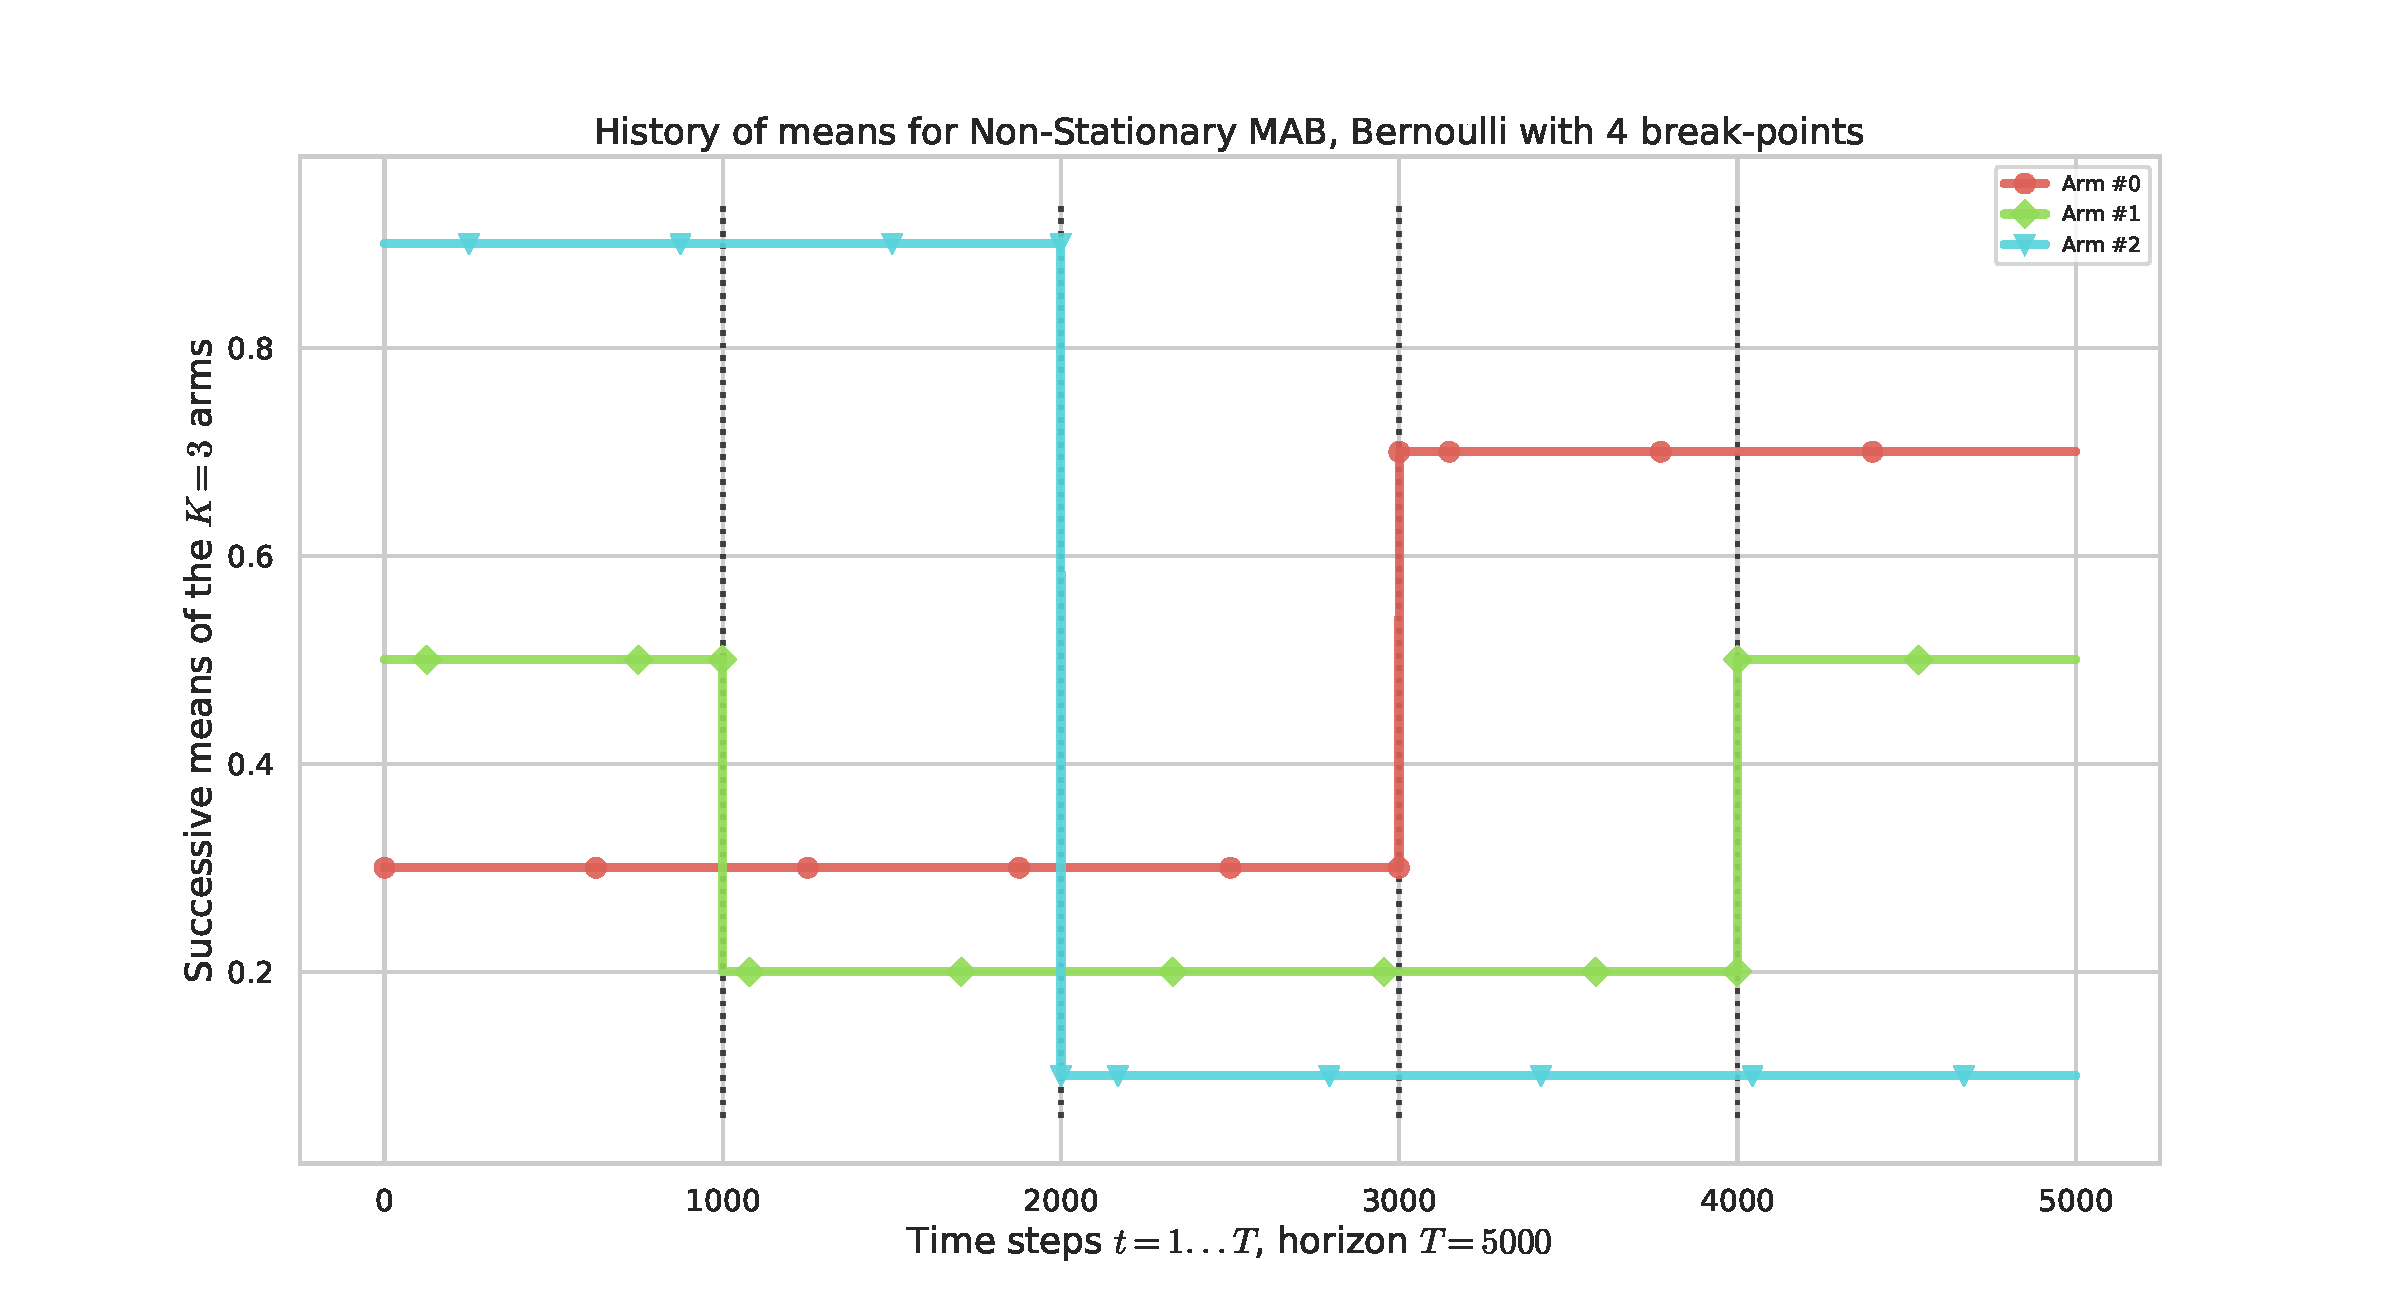
\includegraphics[width=1.15\textwidth]{figures/Problem_1.pdf}
\end{frame}

\begin{frame}[plain]{Results on the first problem}
  \centering
  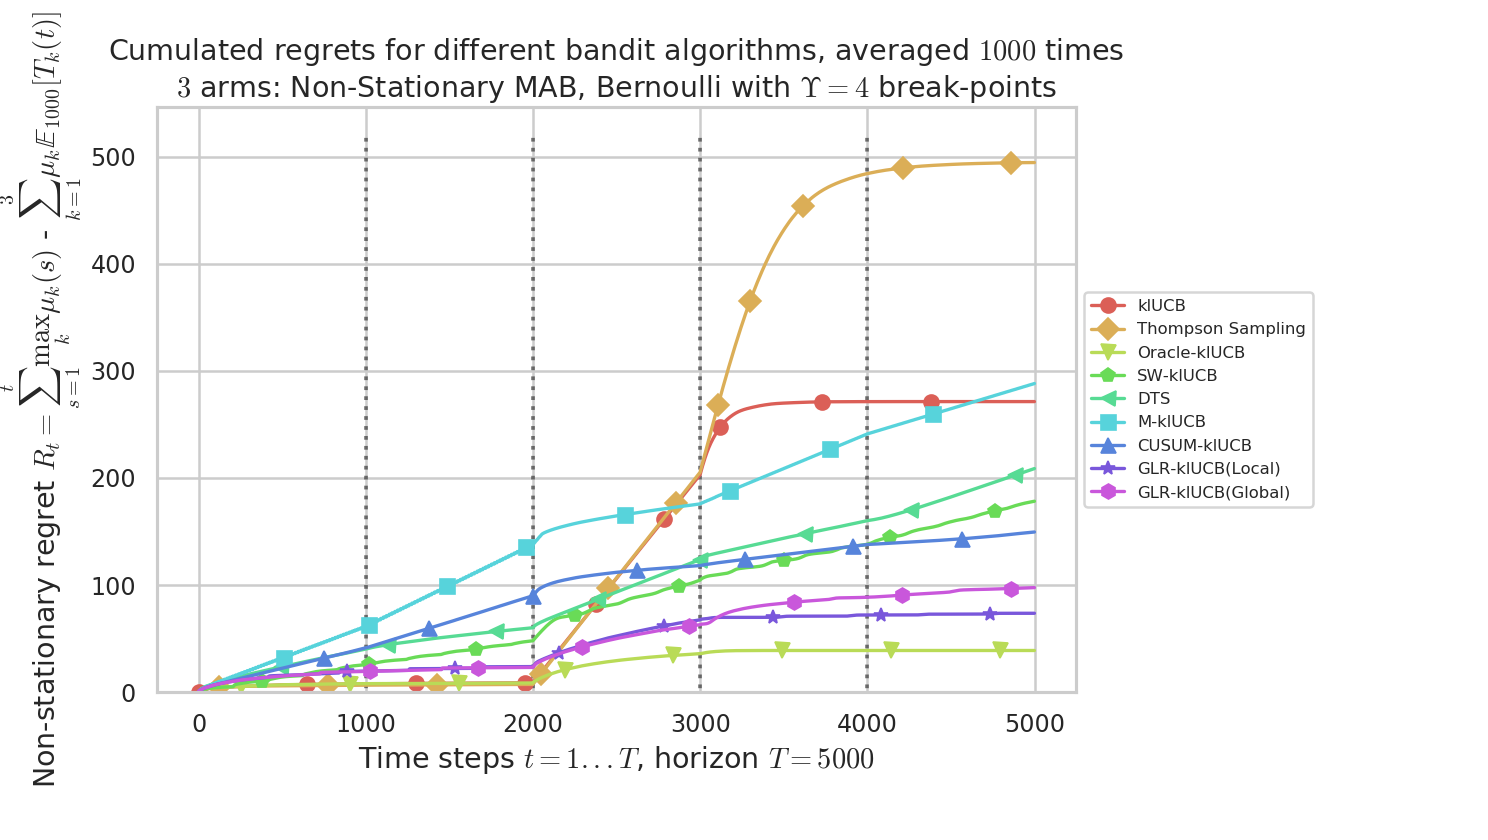
\includegraphics[width=1.15\textwidth]{figures/regret_problem1.png}
  $\implies$ BGLR achieves the best performance among non-oracle algorithms!
\end{frame}


\begin{frame}[plain]{Second problem: only global changes}
  \centering
  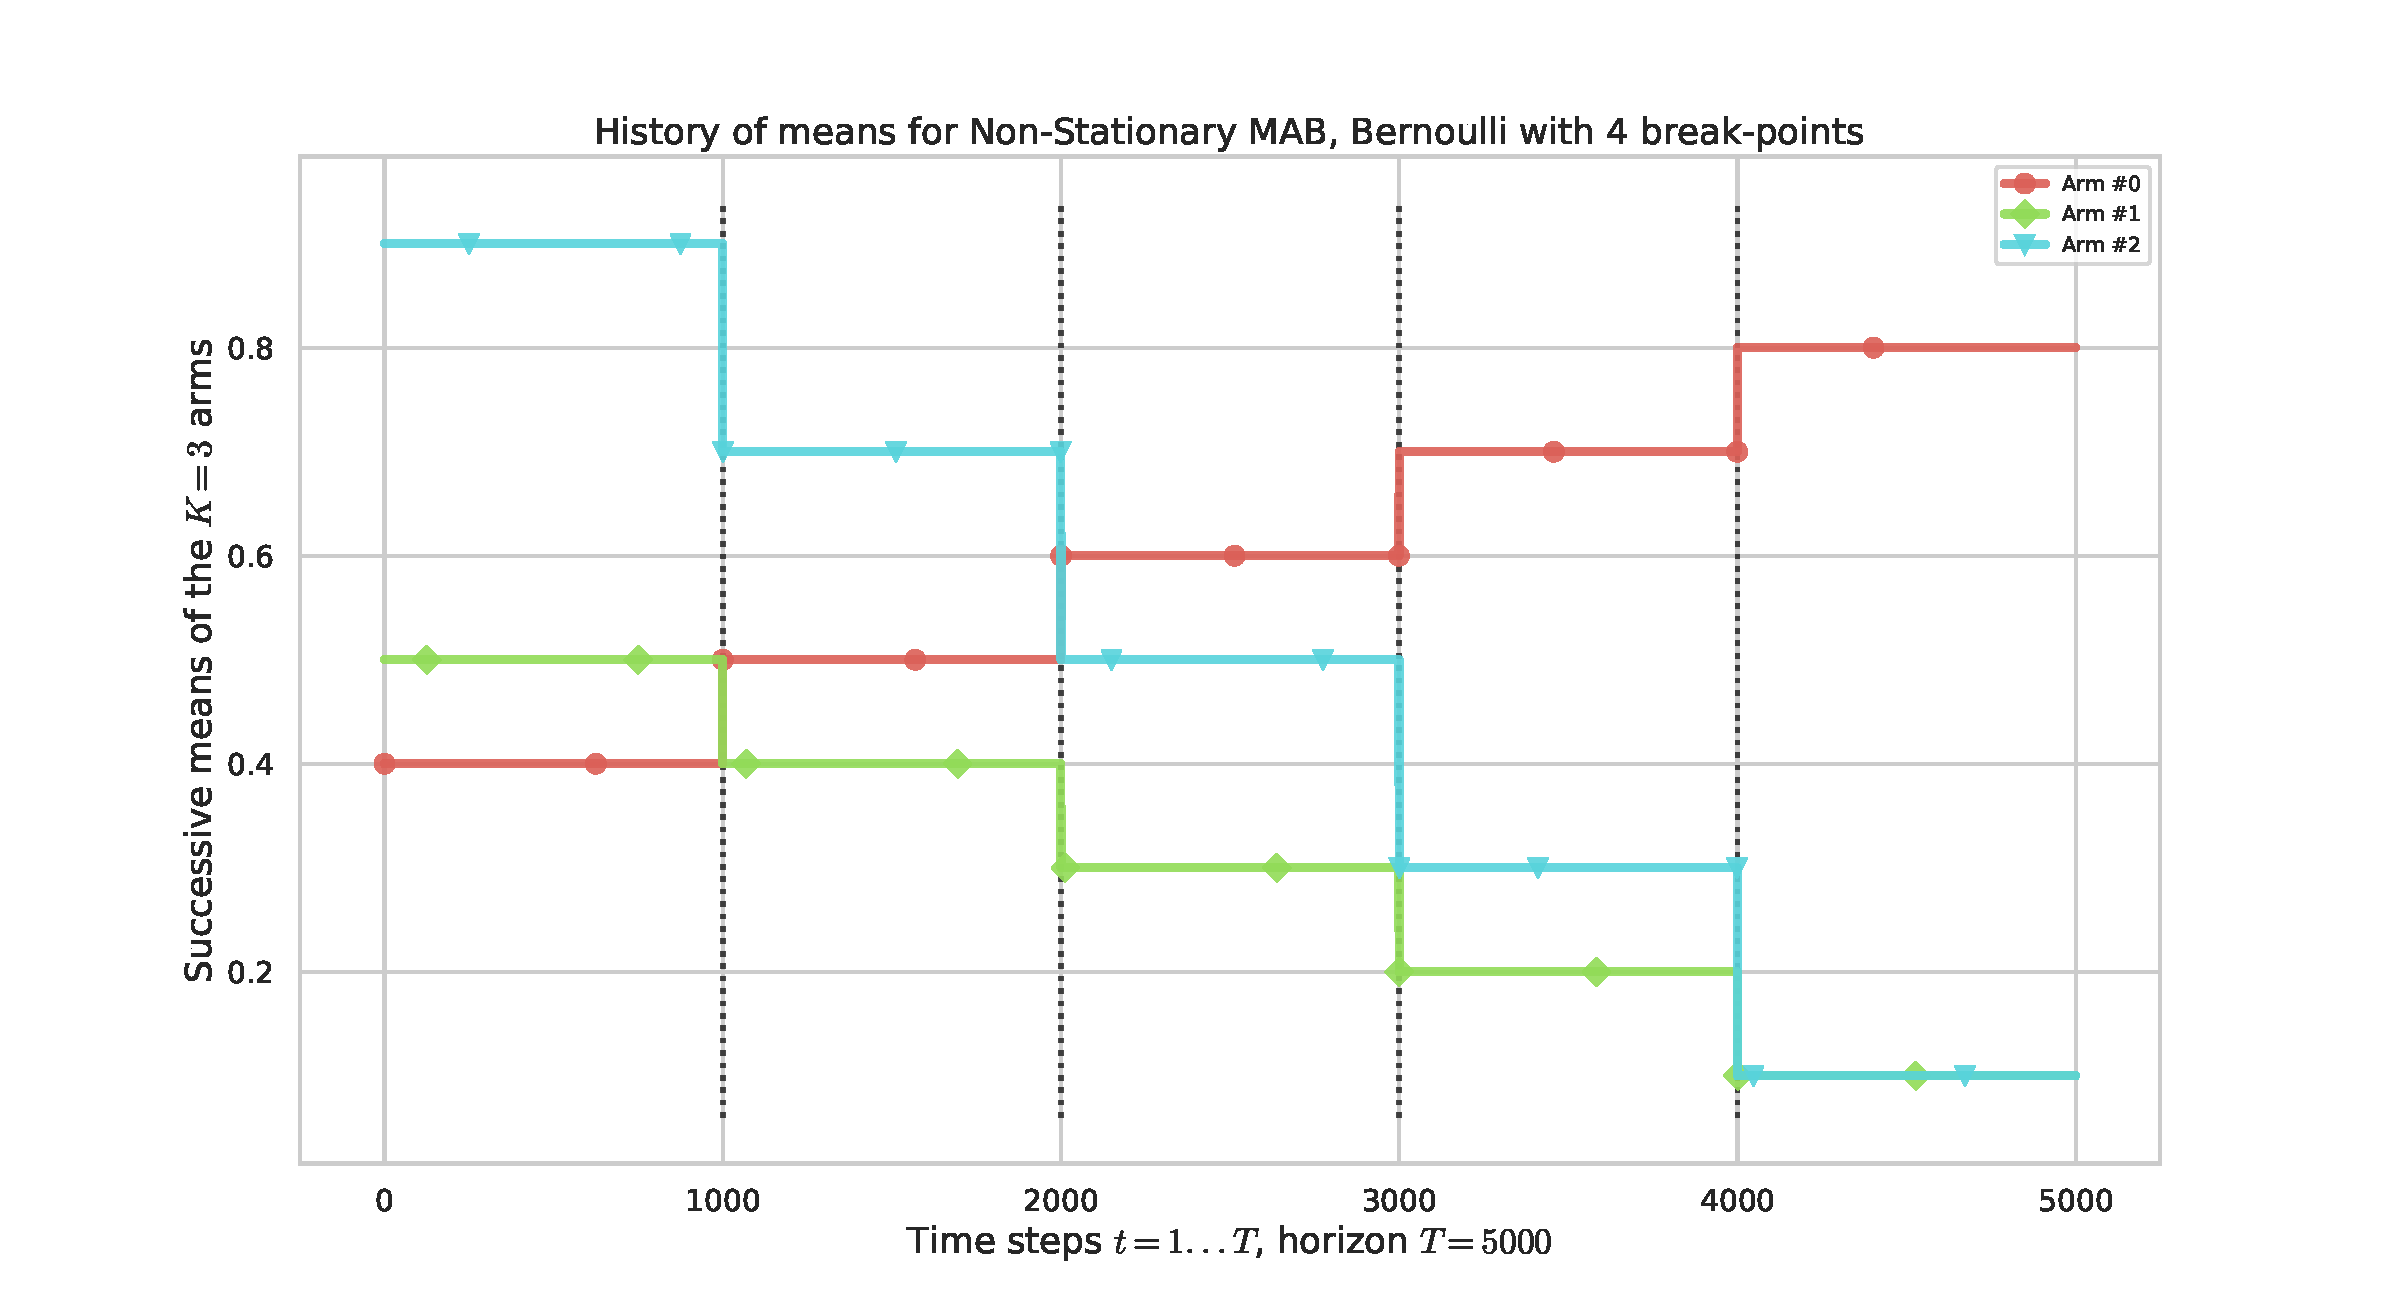
\includegraphics[width=1.15\textwidth]{figures/Problem_2.pdf}
\end{frame}

\begin{frame}[plain]{Results on the second problem}
  \centering
  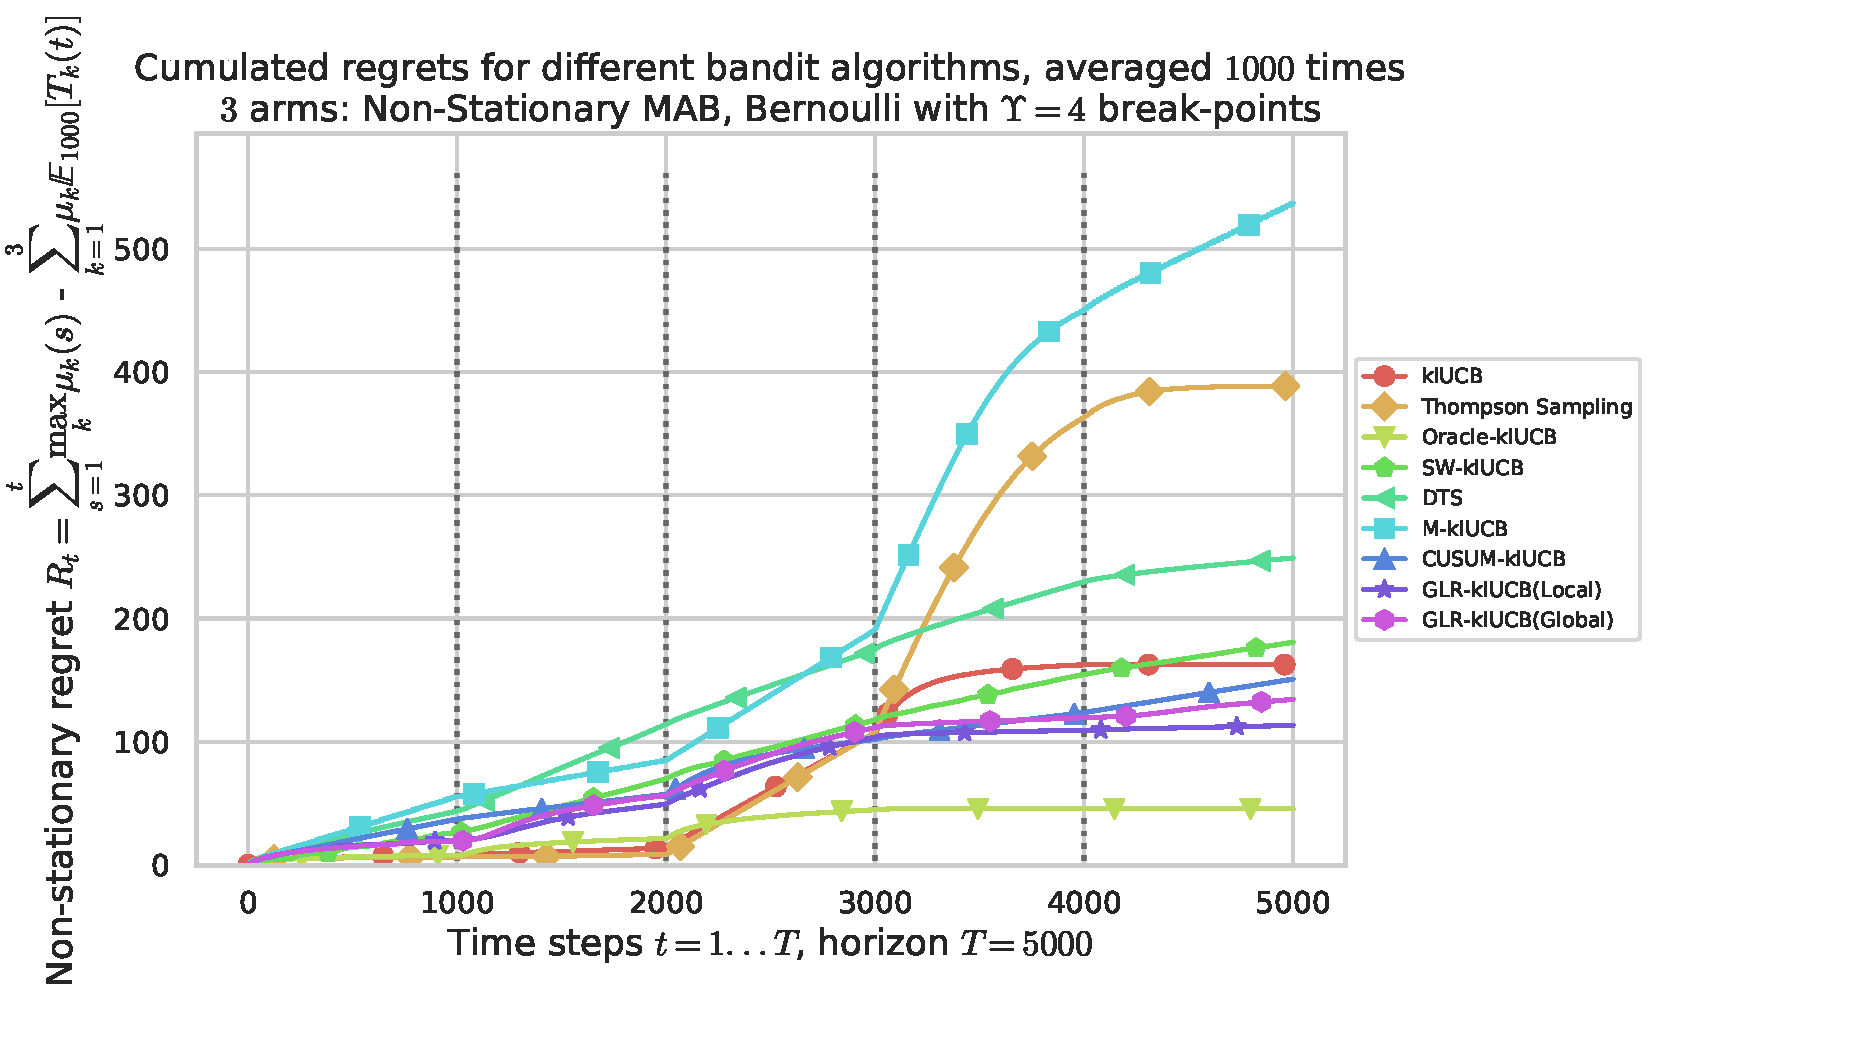
\includegraphics[width=1.15\textwidth]{figures/regret_problem2.pdf}
  $\implies$ BGLR again achieves the best performance!
\end{frame}


\begin{frame}[plain]{Third problem: non-uniform lenghts of stationary intervals}
  \centering
  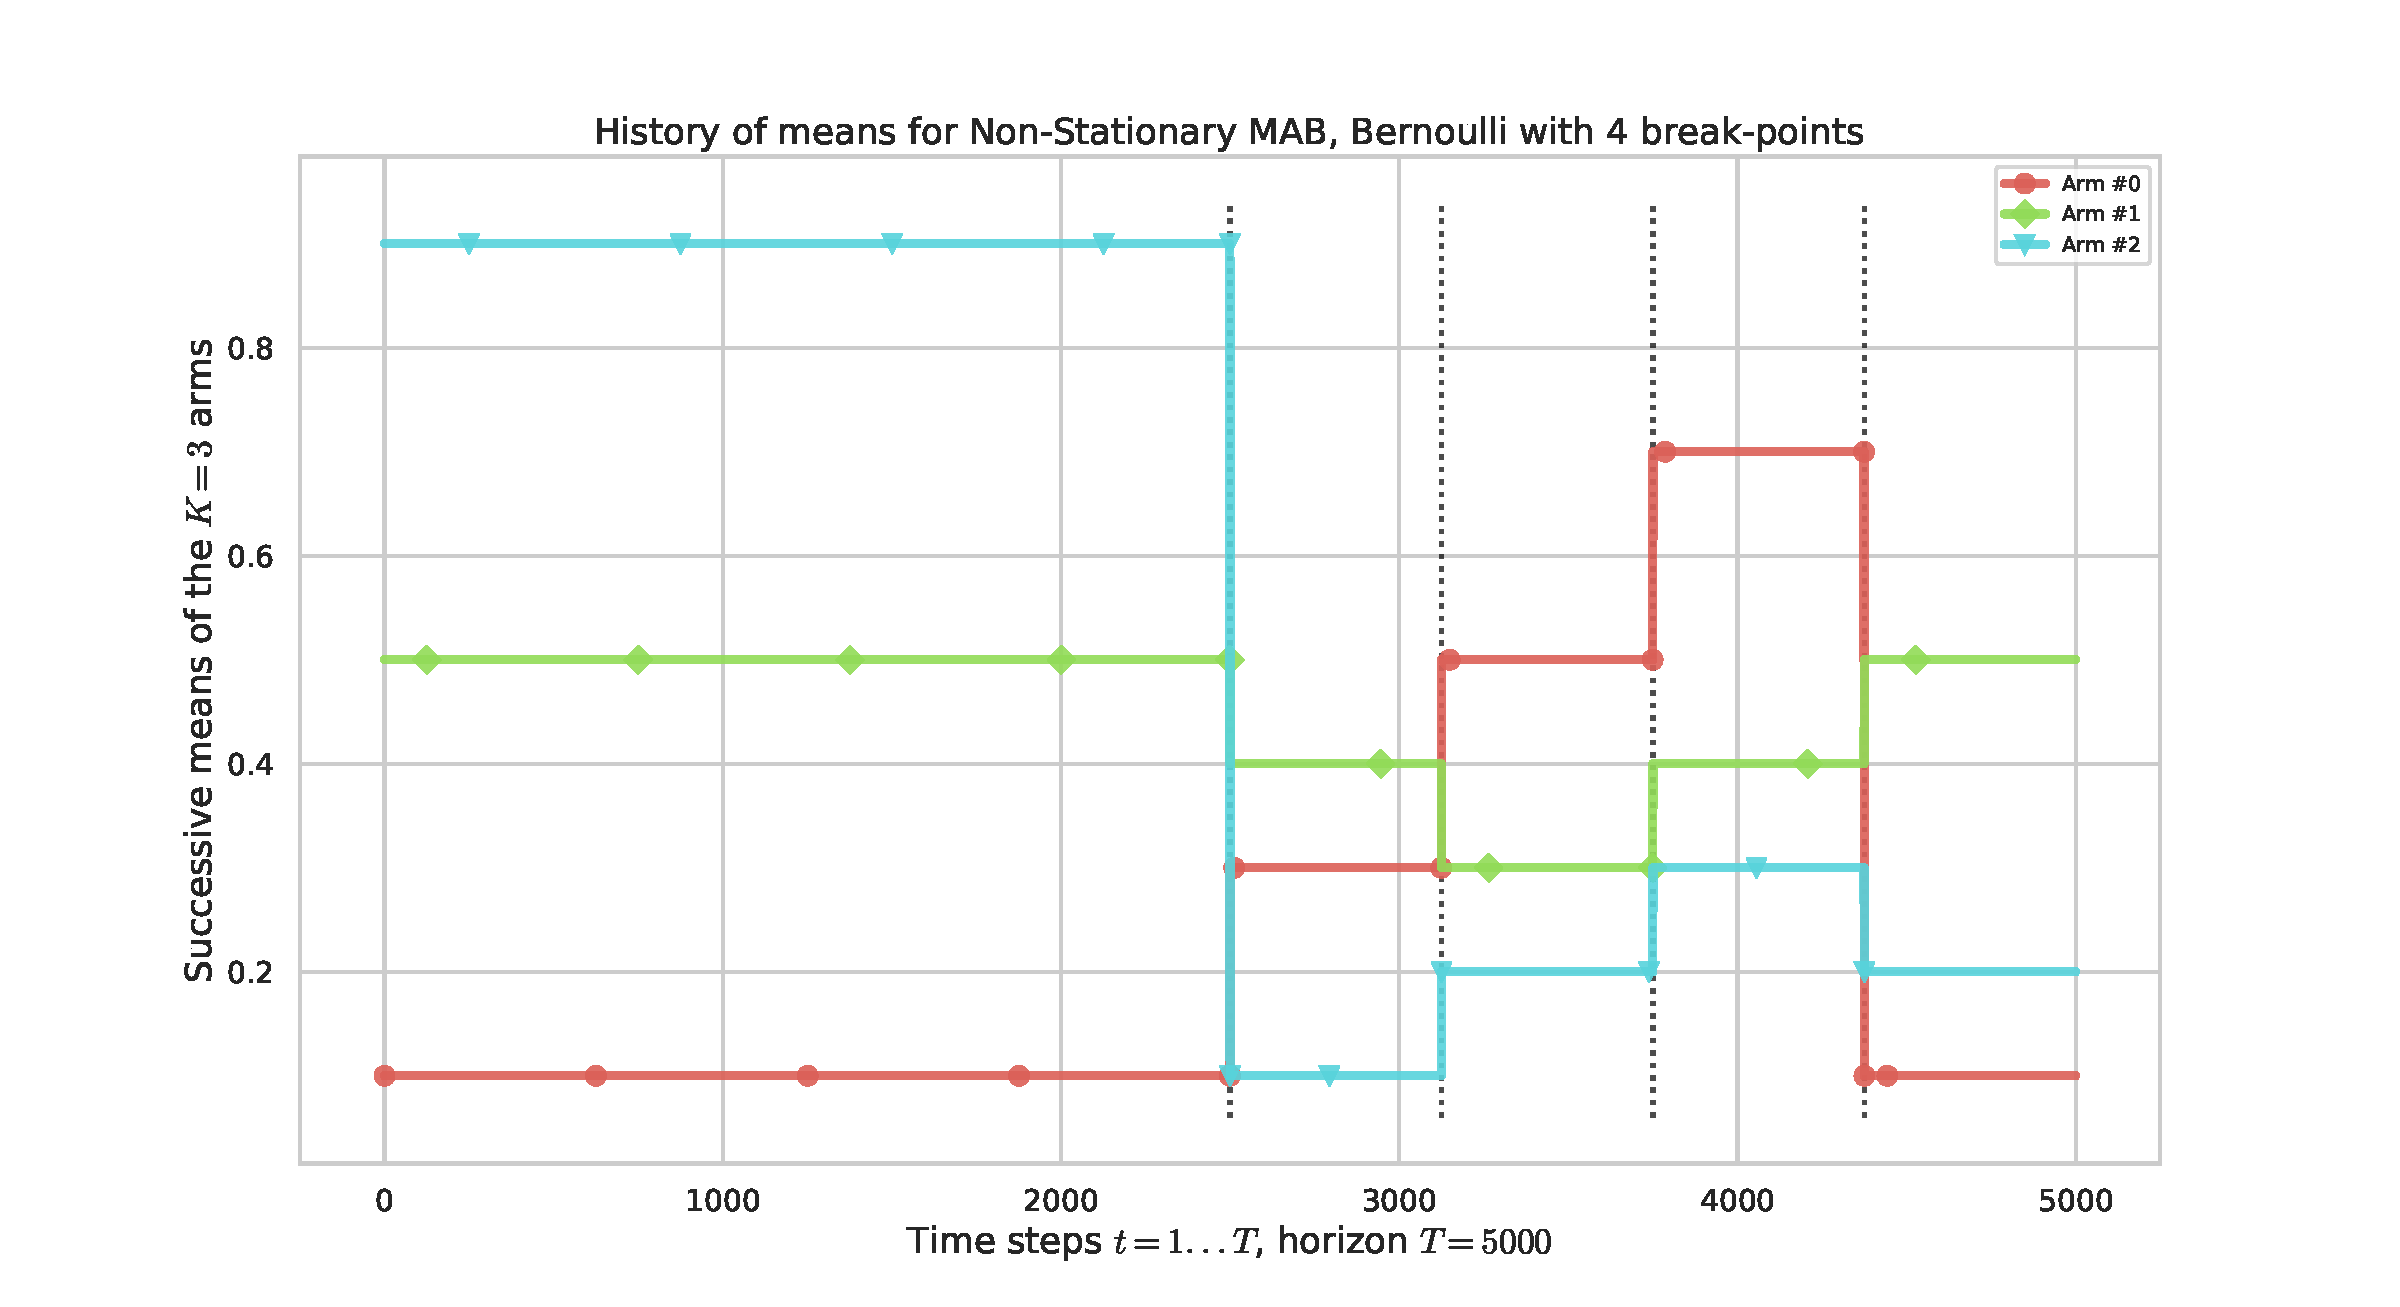
\includegraphics[width=1.15\textwidth]{figures/Problem_4.pdf}
\end{frame}

\begin{frame}[plain]{Results on the third problem}
  \centering
  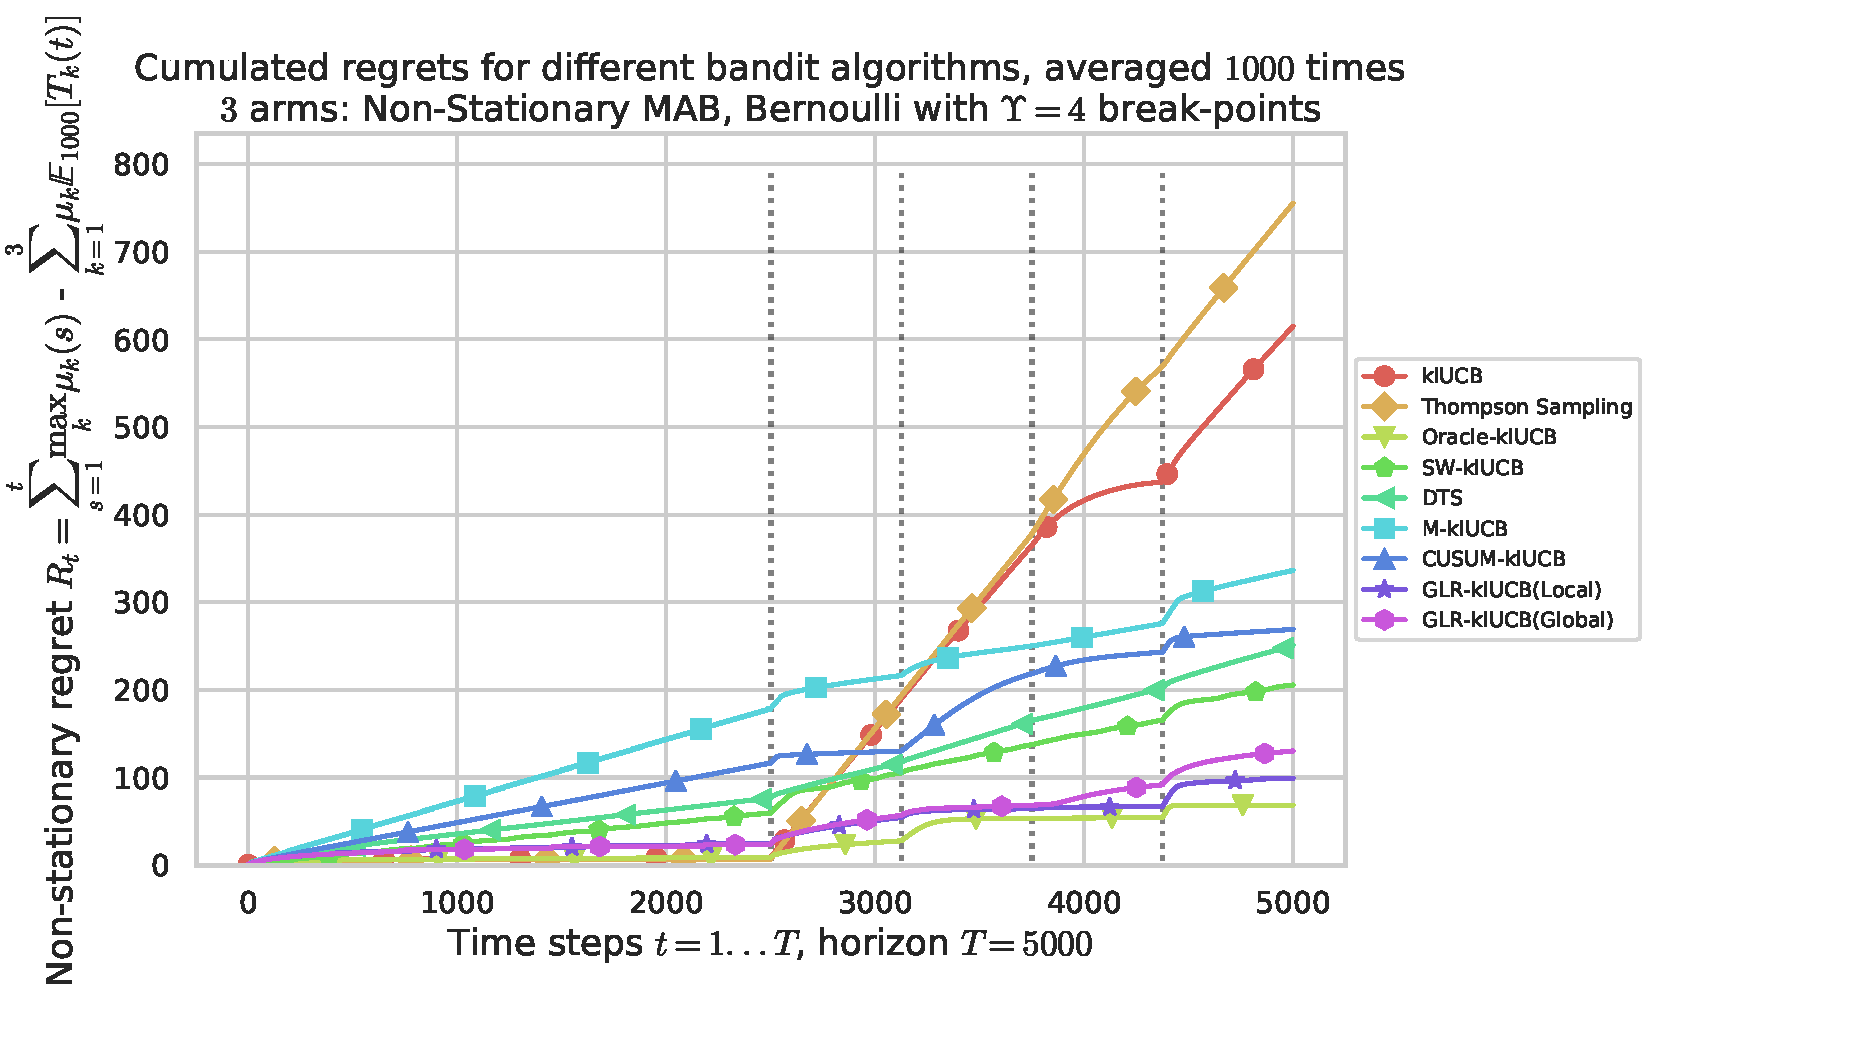
\includegraphics[width=1.15\textwidth]{figures/regret_problem4.pdf}
  $\implies$ BGLR achieves the best performance among non-oracle algorithms!
\end{frame}


\begin{frame}{Interpretation of the simulations}

  \begin{block}{Conclusions in terms of regret}
    \begin{itemize}
      \item
      Empirically we can check that the \alert{BGLR test is efficient}:
      \begin{itemize}\tightlist
        \item
        it has a \alert{low false alarm probability}
        \item
        it has a \alert{small delay} if the stationary intervals are long enough
      \end{itemize}
      And this is ture even if the hypotheses of our analysis are not satisfied!
      \item
      Using the kl-UCB policy gives very good performance
    \end{itemize}
    $\implies$ Our algorithm (BGLR test + kl-UCB) achieves state-of-the-art performance!
  \end{block}

  \begin{block}{What about the efficiency in terms of time and memory?}
    \begin{itemize}
      \item \textbf{Memory:}
      Our algorithm is as efficient as other state-of-the-art strategies!
      (memory $= \mathcal{O}(K \max \text{duration of stationary intervals}})$)
      \item \textbf{Time:}
      But it is costly!
      $\hookrightarrow$ we propose two numerical tweaks to speed it up, see the long version on
      \href{https://hal.inria.fr/hal-02006471}{\textcolor{blue}{HAL-02006471}}
      and
      \href{https://arxiv.org/abs/1902.01575}{\textcolor{blue}{arXiv:1902.01575}}
    \end{itemize}
  \end{block}

\end{frame}



\section{\hfill{}Conclusion\hfill{}}
\subsection{}

\begin{frame}{Conclusion}

\begin{center}
  \begin{LARGE}
    {\Fontify Thanks for your attention .}
    \Smiley[0.9]
  \end{LARGE}
\end{center}

\begin{center}
  \begin{LARGE}
    Questions \& Discussion ?
  \end{LARGE}
\end{center}

\end{frame}

\end{document}
